\chapter{Discussion} \label{sec:discussion}

In Chapters \ref{sec:proximate}, \ref{sec:intermediate}, and \ref{sec:ultimate} we have toured through a sprawling menagerie causal factors associated with evolvability.
These factors included aspects of internal structures of biological organisms (e.g. modularity), the processes that gives rise to the phenotypic structures observed in mature biological organisms (e.g. exploratory growth) the constitution of the environments biological organisms inhabit (e.g. fitness degeneracy), interplay between the structure of biological organisms and the environment (e.g. plasticity), and specific evolutionary processes through which complexity is thought to emerge (e.g. duplication and divergence).
This expedition traveled through a wide range of explanatory scope --- we discussed causal factors related to the immediate physical forms of biological organisms (Chapter \ref{sec:proximate}), causal factors related to overarching design patterns associated with biological organisms (Chapter \ref{sec:intermediate}), and, finally, Chapter \ref{sec:ultimate} reviewed causal factors rooted in the fundamental characteristics of organisms and their environments.
Despite the broad nature of the survey presented in Chapters \ref{sec:proximate}, \ref{sec:intermediate}, and \ref{sec:ultimate}, it does not constitute an exhaustive presentation of factors related to evolvabiltiy.
However, this survey is broad enough to begin to appreciate broader patterns among the factors that contribute to evolvability. 
This background should also be sufficient to shed light on strategies to promote evolvability practiced in evolutionary computing.

Section \ref{sec:how_understand} aims to synthesize overarching theoretical perspective on evolvability from the organizational scheme presented in Chapters \ref{sec:proximate}, \ref{sec:intermediate}, and \ref{sec:ultimate}.
Section \label{sec:how_get} leverages the analysis performed in Section \ref{sec:how_understand} to identify strategies to promote evolvability in an evolutionary computing setting and describes several efforts to promote evolvability from the evolutionary computing literature.


\section{How Should We Understand Evolvability?} \label{sec:how_understand}

As we have seen in Chapters \ref{sec:proximate}, \ref{sec:intermediate}, and \ref{sec:ultimate}, evolvability is a diffuse concept with multiple causality.
Recall that at the most fundamental level, as introduced in Chapter \ref{sec:definition}, evolvability stems from a the availability of heritable variation that is viable.
Recall, also, the two major elements are at play in relation to evolvability: an ability to readily produce diverse heritable phenotypic variation and a bias towards viable variation.
Chasing evolvability further down the rabbit hole, the chain of causality rapidly branches out to a diverse set of interconnected factors;
% Figure \ref{fig:mindmap} visualizes the relationships between evolvability, intermediate causal factors, and ultimate causal factors.
% Individual concepts are depicted as nodes.
% Relations between concepts are depicted with arrows, with green triangle-tipped arrows indicating a promotional relationship and red flat-tipped arrows indicating an inhibitory relationship.
% This diagram traces influence of concepts directly upon another, indicated by connections between nodes, and influence of concepts on relationships between concepts, indicated by connections between a node and the midpoint of another connection. Table \ref{table:intext} serves as a companion to Figure \ref{fig:mindmap}, cataloging where these information on these relationships can be found in the text.

% \begin{samepage}
% \begin{figure}[!htbp]
  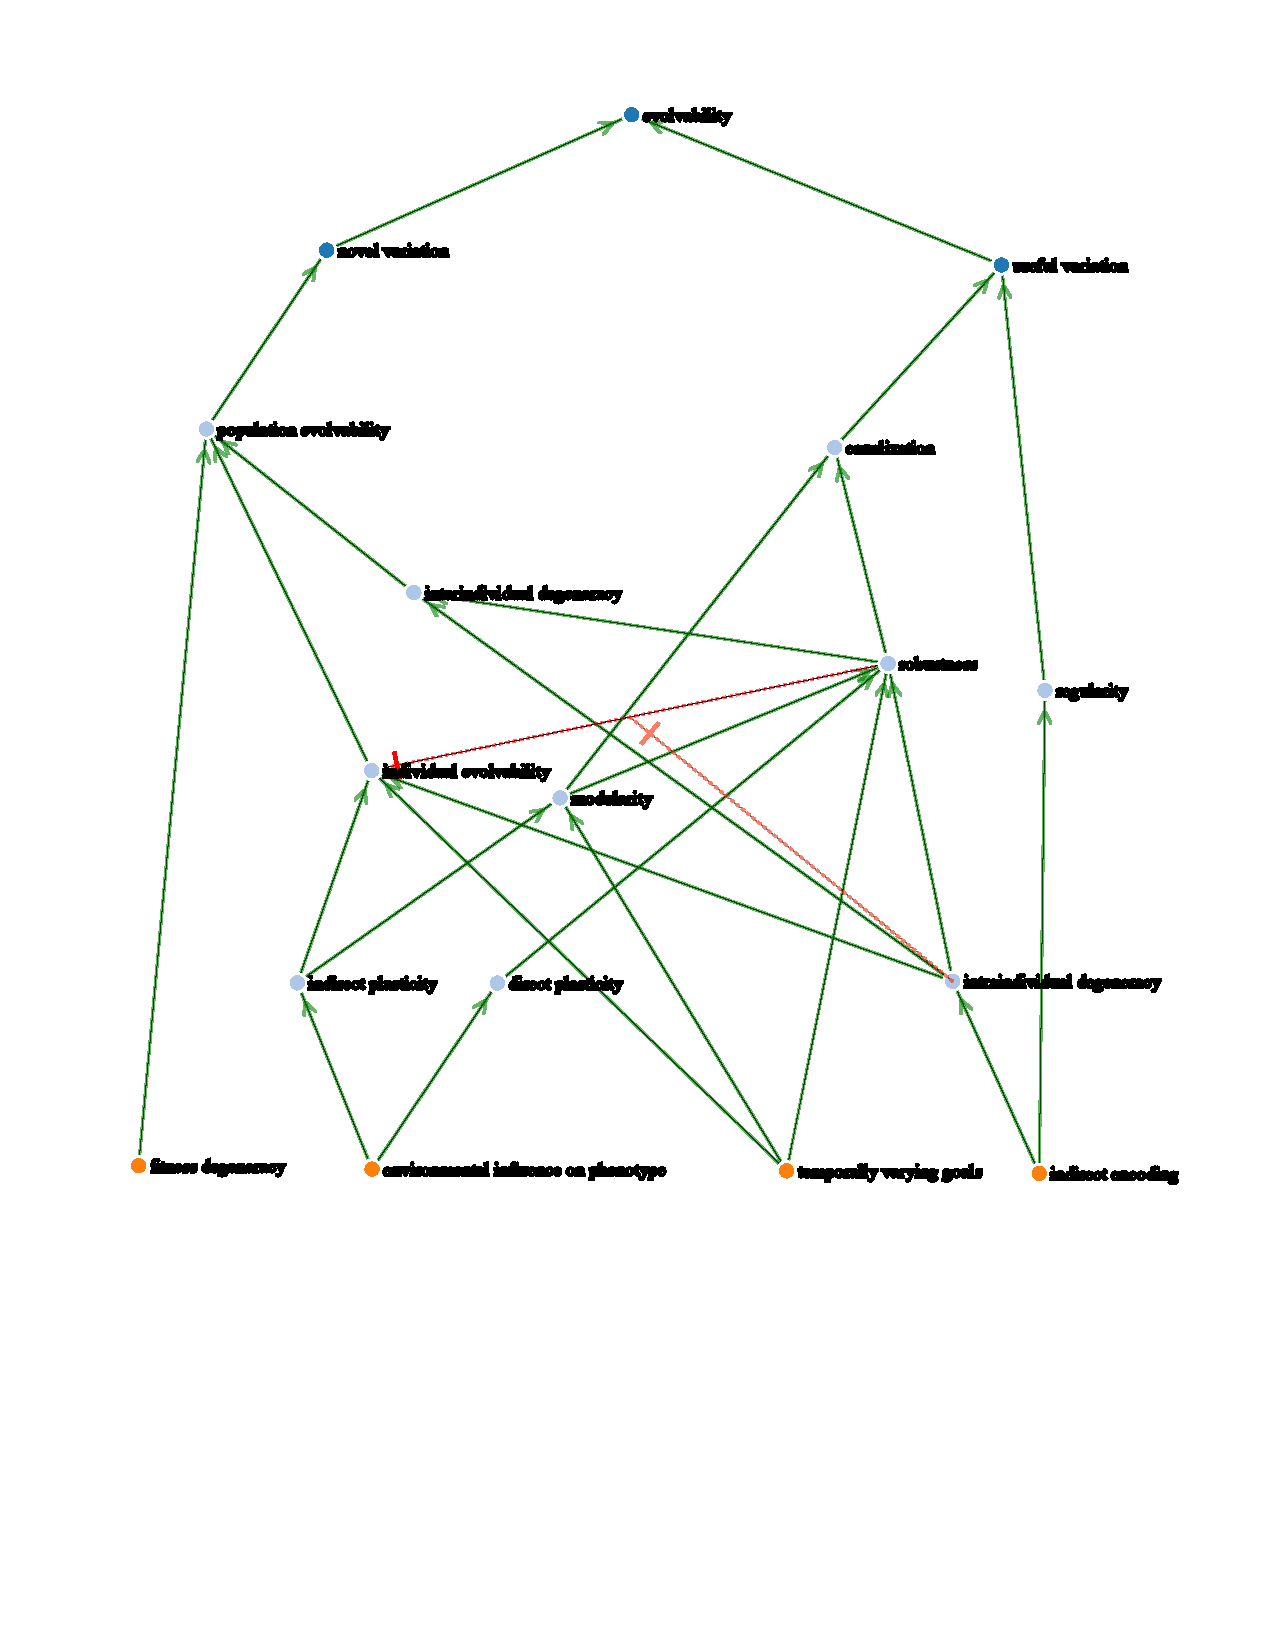
\includegraphics[width=\textwidth]{img/mindmap}
  \captionsetup{singlelinecheck=off,justification=raggedright}
  \caption[Schematic of Interplay between Concepts Related to Evolvability]{A graphical illustration of how causal factors related to evolvability interact. Green solid arrows indicate promotion while red dashed T's indicate suppression. Ultimate causal factors are depicted with a triangular glyph. Intermediate causal factors are depicted with a square glyph. Evolvability and its two major conceptual components are drawn with circular glyphs. Table \ref{table:index} lays out where these relationships are described in the text. Blue asterisks indicate terminology unique to this work.}
     \label{fig:mindmap}
\end{figure}
% \printindex[mindmap]{}
% \end{samepage}

% Figure \ref{fig:mindmap} paints an elaborate portrait of the forces at play behind evolvability picture of the theoretical underpinnings of evolvability.
evolvability stems from a dense web of interactions between many concepts.
% To aid our analysis, let us take a closer look at sub-components of this nexus of causality.
% Figure \inputandref{mindmap_analysis} presents several diagrams that isolate subsets of the theoretical components that promote evolvability to aid analysis of certain aspects of evolvability.
% Figure \ref{subfig:heritable_variation} highlights concepts that promote heritable variation, one of the two primary aspects of evolvability.
% Temporally varying goals, plasticity, and degeneracy appear to be important concepts that promote heritable variation.
% Figure \ref{subfig:viable_variation} highlights concepts that promote viable variation, the other primary aspect of evolvability.
% Canalization and regularity are the most immediate causes of evolutionary bias towards viable variation.
% The concepts of robustness, plasticity, modularity, individual degeneracy, and temporally varying goals contribute indirectly to evolutionary bias towards viable variation.
% Subfigures \ref{fig:mm_tvg}, \ref{fig:mm_environmental_influence}, \ref{fig:mm_indirect_encoding}, and \ref{fig:mm_fitness_degeneracy} isolate concepts related to each ultimate causes of evolvability: temporally varying goals, environmental influence on phenotype, indirect encoding, and fitness degeneracy.
 
%As can be appreciated from Figure \ref{fig:mindmap}, 
The causal factors related to evolvability do not readily lend themselves to to being cleanly teased apart.
However, the proximate-intermediate-ultimate conceptual framework does provide some useful insight into the overall causal framework behind evolvability through the lens of the genotype-phenotype and phenotype-fitness mappings.
Although not cut-and-dried, proximate causes of evolvability tend to be more closely associated with the genotype-phenotype mapping (development).
Ultimate causality is connected to both the genotype-phenotype (development) and the phenotype-fitness (fitness) mappings.
Intermediate causal factors fall in between the intermediate and ultimate groups of causal factors, providing intriguing avenues for selection to act on the genotype-phenotype mapping. That is, intermediate causal factors provide a mechanism for selection for certain characteristics in the genotype-phenotype mapping.

To begin to understand the role proximate factors play in relation to other causal factors, let us begin by developing an understanding of how these proximate factors fit together as a group.
A cursory inspection reveals that this grouping of proximate factors falls into two major categories. 
Duplication and divergence, complexification, weak linkage, and the accumulation of hidden genetic variation are mechanisms that act on a population over evolutionary time (i.e. over the course of multiple generations).
New phenotypic traits emerge from refinement of existing traits, duplication and modification of existing traits, the establishment of novel interaction between subsystems or through enabling (rather than instructive) signaling, and sensitization to previously hidden accumulated genetic variation.
Exploratory growth, developmental constraint are mechanisms that act on the phenotype during the lifetime of an individual (i.e. over the course of the developmental process).
Components of the organism exhibit adaptivity during the developmental process, reacting to the state of other components and the developmental environment so otherwise independent phenotypic traits are synchronized.
The nature of the developmental process governs how genotypic information manifests in the phenotype.

Although the collection of concepts deemed proximate contributors to evolvability are highly diverse, they might succinctly be described as patterns of how phenotypic features emerge through the developmental and evolutionary processes.
All of these concepts ultimately boil down to the genotype-phenotype mapping, the manner in which phenotypic information is stored in the genome.
The intimate intertwining of the genotype-phenotype mapping observed in biology and exploratory growth and developmental constraint, which act over developmental time, can be readily appreciated.
The connection between the proximal traits that act over evolutionary time and the genotype-phenotype mapping is a bit subtler.
All four of these proximate contributors to evolvability --- duplication and divergence, complexification, weak linkage, and hidden genetic variation --- are related to the addition of new phenotypic information to the genome.
Duplication and divergence leverages existing information in the genome to jump start phenotypic innovation.
Complexification is enabled by the ability of the genome to assimilate new information describing a phenotypic trait in increasing detail.
Weak linkage is a phenotypic adaptation --- propensity to use enabling over instructive signaling --- that reduces the amount of information that must be added to the genome to establish regulatory links between separate systems.
Hiding segments of the genome from phenotypic expression allows for the accumulation of novel genetic information in a population that can then be exposed through sensitizing mutation.
The manner in which phenotypic information is stored in the genotype is inherently related to the genotype-phenotype mapping, hence the connection between these concepts and that mapping.
The Baldwin Effect sits somewhat apart from other proximate causal factors related to evolvability.
Although influencing the genotype-phenotype mapping like other proximate causal factors, the Baldwin Effect is also tied to the phenotype-fitness mapping as it essentially performs local search in phenotypic space for fitness peaks.
For the most part, with this slight exception, proximate causes of evolvability can be understood as acting on the genotype-phenotype mapping. 

Ultimate causality, in contrast, exhibits significant ties to both the genotype-phenotype and the phenotype-fitness mapping.
Temporally varying goals and fitness degeneracy explicitly describe aspects of the fitness function, its fluctuation over evolutionary time and its permissibility for phenotypic diversity. Environmental influence on the phenotype, like the Baldwin Effect, has a foot in both mappings.
Environmental influence affects the genotype-phenotype mapping, allowing different phenotypic outcomes to be observed from any particular genotype. 
However, in the case of indirect plasticity, environmental influence can signal information about the phenotype-fitness mapping to the genotype-phenotype mapping --- namely, which phenotypic outcome would be favored in terms of fitness.
Indirect encoding, of course, is directly related to the genotype-phenotype mapping and not to the phenotype-fitness mapping.
In the next section, we will see how our presentation of the proximate-intermediate-ultimate organizational scheme in terms of the genotype-phenotype and the phenotype-fitness mappings will inform strategies to promote evolvability in evolutionary computing.

\section{How Do We Get Evolvability?} \label{sec:how_get}

A maximally biologically-plausible model would explicitly account for solely on ultimate causal factors, listed in Chapter \ref{sec:ultimate}, to promote evolvability.
It is thought that in nature, the proximate and intermediate causal factors described in Chapters \ref{sec:intermediate} and \ref{sec:proximate} manifest in biological organisms as a result of the evolutionary process, not as a precursor to it. 
As we can see from our analysis, the fundamental assumptions of ultimate causality are related both to the genotype-phenotype mapping and the phenotype-fitness mapping. 
Proximate causes are, in contrast, primarily tied to the genotype-phenotype mapping.
In nature, where the developmental process (i.e. the genotype-phenotype mapping) is largely controlled by the genotype, we would expect to observe proximate causes of evolvability --- associated most strongly with the genotype-phenotype mapping --- to emerge through the evolutionary process. 

However, allowing the developmental process to be fundamentally controlled by the genotype is easier said than done in evolutionary computing.
Attempting to model an arbitrary level of biological realism is simply computationally intractable  \cite[p 354]{Downing2015IntelligenceSystems}.
How can proximate causes of evolvability be realized at a reasonable computational cost?
From a practical standpoint, explicit scaffolding (i.e. a development scheme with significant manually designed aspects) is an almost certain necessity.
Simulating a digital system that even comes near to directly reproducing the developmental processes observed in biology is currently well outside the scope of computational feasibility.
Instead researchers can attempt to devise models of the genotype-phenotype mapping that shake out desirable properties of the genotype-phenotype mapping associated with proximate causes of evolvability at a reasonable computational cost.

Another shortcut to evolvability available to researchers willing to depart from strict adherence to the biological metaphor can be found among the intermediate causes of evolvability.
Intermediate causal factors include modularity, canalization, robustness, individual evolvability, intraindividual degeneracy, and interindividual degeneracy.
In nature, these intermediate contributors to evolvability are also qualities gained by evolving organisms through the evolutionary process, not built a priori into an evolving system.
In concrete terms, this means that these traits would be essentially absent in a randomly generated population at generation zero but might develop as evolution proceeds under the right conditions.
Intermediate causal factors tend to be less prone to direct manual instantiation compared to their proximate cousins because intermediate causal factors are largely not explicit components of the developmental process.
However, that does not mean that intermediate causal factors are ill-defined or unobservable. 
Especially in digital organisms, these traits can be directly quantified (usually in the context of a single individual).
Reisinger et al. quantify canalization by measuring the rate at which random mutation degrades fitness \cite{Reisinger2007AcquiringRepresentations}.
A domain-specific metric for modularity has been developed by \cite{Kashtan2005SpontaneousMotifs}.
The ability to quantify these traits associated with intermediate causality allows direct selection for them.\footnote
{It should be noted that intraindividual degeneracy, which manifests in differences between individuals rather than within a single individual, is slightly different from the other listed intermediate contributors in this regard.
However, selection to directly promote intraindividual degeneracy might nonetheless be possible by divergent selection to reward novel neutral phenotypic and/or genotypic variation.}
That is, individuals that exhibit a desirable trait related to evolvability, such as modularity or intraindividual degeneracy, could be explicitly chosen to populate the next generation. The hope would be to observe these traits become more prevalent over evolutionary time.

Our analysis of strategies to promote evolvability has focused on two major ideas: the genotype-phenotype mapping (development) and the phenotype-fitness mapping (selection). The proximate-intermediate-ultimate framework has shed light on strategies targeting both mappings, in particular how each can be accomplished both inside and outside of strict adherence the biological metaphor. Possible strategies to promote evolvability can be summarized as:
\begin{itemize}
\item taking a broader view of selection 
\begin{itemize}
\item more open-ended environments that exhibit fitness degeneracy and temporal change
\item non-objective-based selection mechanisms
\end{itemize} 
\item adopting a more nuanced view of the developmental process
\begin{itemize}
\item allowing for a more biologically plausible developmental process that incorporates environmental influence on the phenotype and allows a high level of genetic control of the developmental process
\item manually building scaffolding for the developmental process to incorporate aspects of proximate contributors to evolvability at a feasible computational cost
\end{itemize}
\end{itemize}
Since the conception of the field of evolutionary algorithm design efforts under each of these banners have already had transformative effects on the field. Such efforts are reviewed next in Sections \ref{sec:representations} and \ref{sec:selection}. 

At first blush, it very well might seem that these efforts to apply a broader, more nuanced view of evolution to the evolutionary algorithm amount to abandoning abandoning practical applications of the evolutionary algorithm.
After all, these first components of the path forward for evolutionary computing entails moving away from exclusive explicit selection for the ability of a digital organism to fulfill a desired function.
The second involves incorporation of more nuanced developmental processes, efforts that might not seem to directly relate to the ability of a mature phenotype to serve a desired function and instead merely appear to be an extravagant pretense to biological realism where ``the complexity of the model dwarfs that of the task...'' \cite[p 354]{Downing2015IntelligenceSystems}.
However, the exact opposite is the case --- these efforts aim to unlock the power of evolutionary innovation, so that it may be better harnessed for applied ends.
Indeed, these ideas have been adopted in applied scenarios where greater task performance is desired and have yielded it \cite{Cheney2013UnshacklingEncoding, Mengistu2016EvolvabilityIt, Reisinger2007AcquiringRepresentations, Lehman2008ExploitingNovelty}.
The central question that evolutionary algorithms researchers confront seems to be: at what level of abstraction can a biologically-inspired route to profound and useful innovation via evolution be realized?
At the heart of the matter, evolutionary algorithm researchers a re challenged to sort out what biological factors are important to the evolutionary process and devise clever ways to model them without the undue computational cost of a naive approach.
The path forward will depend heavily on continued rigorous experimental work to suss out the constellation of causality behind evolvability in biological systems and digital models.
It is hoped that this experimental work, guided and motivated by theoretical analysis, will ultimately yield stronger methodological techniques to promote evolvability in digital systems and, thus, continue to advance the practical utility of evolutionary algorithms in applied settings.
Next, we will look at some examples of existing methodological techniques that have been designed to promote evolvability.

\subsection{Representations} \label{sec:representations}

Genetic representation design in evolutionary computing is typically a domain-specific endeavor.
The manner in which a genotype-phenotype mapping is designed depends on the phenotype space it must map to. However, some design patterns do exist across domains and these are nicely exemplified by work being done in Evolving Artificial Neural Networks (EANNs).
The goal of EANNs are to discover configurations of nodes and connective weights so that cause an artificial neural network to exhibit a desired behavior.
Scalability a key hurdle for EANNs; evolving large artificial neural networks is difficult. 
EANNs have yet to rival the scale and intricacy of their biological counterparts and it is thought that poor genetic encoding is responsible for much of this difficulty \cite{Tonelli2013OnNetworks}.

Perhaps not surprisingly then, researchers have turned to biology to inspire new genetic encoding schemes for EANNs.
On the more literal side of the biological inspiration coin lies Bongard and Pfeifer's artificial ontogeny (AO) system.
In this system, the phenotype is constructed through successive duplication and differentiation of a single virtual cell modulated by simulated diffusion of chemical substances which in turn stem from simulated genetic regulatory networks \cite[p 345]{Downing2015IntelligenceSystems}.
Mouret et al.'s map-based encoding occupies a middle ground in terms of literal interpretation of biological inspiration.
Styled after models of the Basal Ganglia developed by neuroscientists, the map-based model jettisons the individual neuron as the fundamental unit of network composition.
Instead, layers each consisting of an arbitrary number neurons, which are strung together by several pre-defined regular connection schemes (i.e. one to one or one to all), are taken as the fundamental unit of network composition \cite{Mouret2010ImportingGanglia}.

HyperNEAT, a highly influential and ubiquitous encoding in evolutionary computing, lies on the reverse side of the biological inspiration coin --- it exhibits highly abstracted biological inspiration.
HyperNEAT is built off the NEAT encoding scheme developed by Stanley and Miikkulainen \cite[p 324]{Downing2015IntelligenceSystems}.
NEAT is a direct, variable-length encoding for neural networks that reduces omissions and redundancies introduced during crossover by tracking historical markers associated with each gene, in essence implementing a rough approximation of synapsis during meiosis.
HyperNEAT repurposes NEAT to encode a Compositional Pattern Producing Network (CPPN) instead of encoding a neural network.\footnote{
A CPPN is a weighted network of nodes, each of which performs a transformation on its inputs to generate an output --- essentially a neural network where nodes may perform transformations other than the logistic equation. The CPPN at its core is just a mathematical expression that accepts several inputs and generates several outputs.}
The weight of the connection between two nodes in the neural network generated by HyperNEAT is determined by the output of the CPPN fed the coordinates of those two nodes.
The CPPN in essence serves as the genotype in the HyperNEAT scheme.
The activation patterns projected onto the substrate occupied by artificial neurons in the HyperNEAT scheme by the CPPN are analogous to patterns of chemical diffusion that play a key role in directing embryological development \cite[p 339]{Downing2015IntelligenceSystems}.
In the original HyperNEAT concept, artificial neurons were arranged in a simple grid pattern.
Subsequent efforts have been made to implicitly define neuron placement based on CPPN output, allowing for the network to grow in numerical size over evolutionary time \cite{Risi2010EvolvingSubstrate,Risi2010IndirectlyRules'}.

Although great strides have been in developing representational techniques, allowing effective EANNs of much larger scale than before, a lot of ground remains to be covered.
EANNs still fall short of the scale exhibited by biological neural networks.

\subsection{Selection Pressure} \label{sec:selection}

In biological evolution, selection criteria are neither monolithic nor static.
Although single-objective, static selection is perhaps the most intuitive strategy to use in an evolutionary algorithm at first blush, such a selection scheme constitutes a rather simplistic interpretation of the biological metaphor.
A number of recent efforts have leveraged inspiration from selection in biological evolution to great effect.
Researchers have ventured away from static objective-based selection by employing temporally varying goals, selection criteria that change over evolutionary time.
This selection paradigm in evolutionary computing reviewed in Section \ref{sec:tvg}.
Inspired by the abundance of niches in biological environments, Ngyuen et al. performed experiments considering the possibility of evolving towards several objectives at once.
They found that, compared to evolving towards a single objective, defining a large set of fitness criteria and determining selection based on the maximum fitness score obtained under one of those criteria, yielded better quality solutions for each objective \cite{Nguyen2015InnovationLearning}.
In their computational experiment, Ngyuen et al. observed objective switching, where offspring are better suited to a niche distinct from that occupied by their parent, occur at a significant rate.
Mengistu et al. have hypothesized that this niche-inspired approach encourages individual evolvability by rewarding individuals with offspring that are  phenotypically variable enough to jump between objectives \cite{Mengistu2016EvolvabilityIt}.

As suggested in the analysis performed at the open of this section, researchers have also identified several successful selection strategies that depart from strict adherence to the biological metaphor.
Highly notable among these is novelty search.
This selection scheme discards traditional objective-based metrics in favor of selecting for individuals that are the most novel, that are the most distinct from individuals that have already been encountered during evolutionary search \cite{Lehman2008ExploitingNovelty}.
Although not directly consistent with the biological metaphor, it has been suggested that such an approach captures the open-ended nature of novelty search in ways that other selection schemes fail to do.
Surprisingly enough, it has been found that in certain scenarios jettisoning selection for an objective in favor of searching for novelty (and keeping track of the best-performing solutions encountered along the way) can actually lead to better performance in satisfying that objective \cite{Lehman2008ExploitingNovelty}.
Novelty search has been found to promote evolvability: selecting for novelty rewards individuals that create variable offspring \cite{Lehman2011ImprovingSelf-Adaptation}.

More recently, Mengistu et al. demonstrated a scheme where individual evolvability is directly selected for  \cite{Mengistu2016EvolvabilityIt}.
Like novelty search, this selection scheme ignores objective performance when performing selection.
Instead, individuals that create a set of offspring that exhibit the greatest phenotypic diversity amongst siblings are selected for.
Also like novelty search, the best-performing individuals according to the objective function are simply logged along the way.
Although subtle, it is an important point to that these two objective-bucking strategies are not random search. Individuals are instead selected for based upon criteria --- either individual evolvability or novelty --- that specifically aim to facilitate wide-ranging search. 
It is in the course of these wide-ranging journeys through phenotype space that these search strategies encounter solutions that well satisfy the objective.
